\chapter{恢复控制}

\begin{introduction}[期末考试复习提纲]
    \item 故障类型
    \item 备份概念及其类型
    \item 日志定义、事务类型及其恢复操作、先写日志的WAL原则
    \item 检查点概念及其作用
    \item 基本的故障恢复操作
    \item ARIES恢复算法所遵循的原则、所涉及到的重要数据结构、三个恢复阶段
\end{introduction}

\section{故障类型}

故障分为三类:
\begin{enumerate}
    \item \textcolor{red}{事务故障}: 事务运行没有到达预期的终点就被中止.
    \item \textcolor{cyan}{系统故障}: 由于系统错误导致的故障.
    \item \textcolor{blue}{介质故障}: 由于介质错误导致的故障.
\end{enumerate}

\begin{definition}[事务故障]
单个事务的运行没有到达预期的终点就被中止.

分为:
\begin{enumerate}
    \item \textcolor{red}{非预期故障}: 不能由事务程序处理的. 如运算溢出, 发生死锁而被选中撤消该事务.
    \item \textcolor{blue}{预期故障}: 应用程序可以发现的事务故障, 并且应用程序可以让事务回滚. 如转帐时发现帐面金额不足.
\end{enumerate}
\end{definition}

\begin{definition}[系统故障]
又称为\textcolor{red}{软故障}(soft crash). 在硬件故障、软件错误的影响下, 虽引起内存信息丢失, 但未破坏外存中数据.
如CPU故障、突然停电. DBMS, OS, 应用程序等异常终止.
\end{definition}

\begin{definition}[介质故障]
又称为\textcolor{red}{硬故障}(hard crash). 又称磁盘故障, 破坏外存上的数据库, 并影响正在存取这部分数据的所有事务.
如磁盘损坏、磁带损坏. 磁盘的磁头碰撞, 瞬时的强磁场干扰.
\end{definition}

\begin{definition}[恢复]
恢复是把数据库从错误状态恢复到某一正确状态的功能, 从而确保数据库的一致性.

恢复的基本原理是\textcolor{red}{冗余}. 即数据库中任一部分的数据可以根据存储在系统别处的冗余数据来重建.
\end{definition}

\section{备份}

\begin{definition}[转储]
将数据库复制到磁带或另一个磁盘上保存起来的过程.

这些备用数据称为后备(后援)副本.
\end{definition}

转储分为:
\begin{enumerate}
    \item 静态转储. \textit{转储期间不允许对数据库进行任何存取、 修改活动.}
    \item 动态转储. \textit{转储期间允许对数据库进行存取或修改.}
    \item 海量转储. \textit{每次转储全部数据库.}
    \item 增量转储. \textit{每次只转储自上次转储以来发生变化的数据.}
\end{enumerate}

数据库备份 by SQL Server:
\begin{lstlisting}[language=sql]
EXEC sp_addumpdevice 'disk', 'mybackup', 'c:\backup\mybackup.dat';
BACKUP DATABASE mydb TO mybackup
RESTORE DATABASE mydb FROM mybackup
\end{lstlisting}

\begin{lstlisting}[language=sql]
-- 完整备份. 首次备份或初始化备份, 为后续差异备份提供一个基准点.
backup database LJCHEN to MyBKDB with init
-- 差异备份
backup database LJCHEN to MyBKDB with differential
restore database LJCHEN from MyBKDB with norecovery
restore database LJCHEN from MyBKDB with norecovery
\end{lstlisting}

MySQL备份:
\begin{figure}[H]
    \centering
    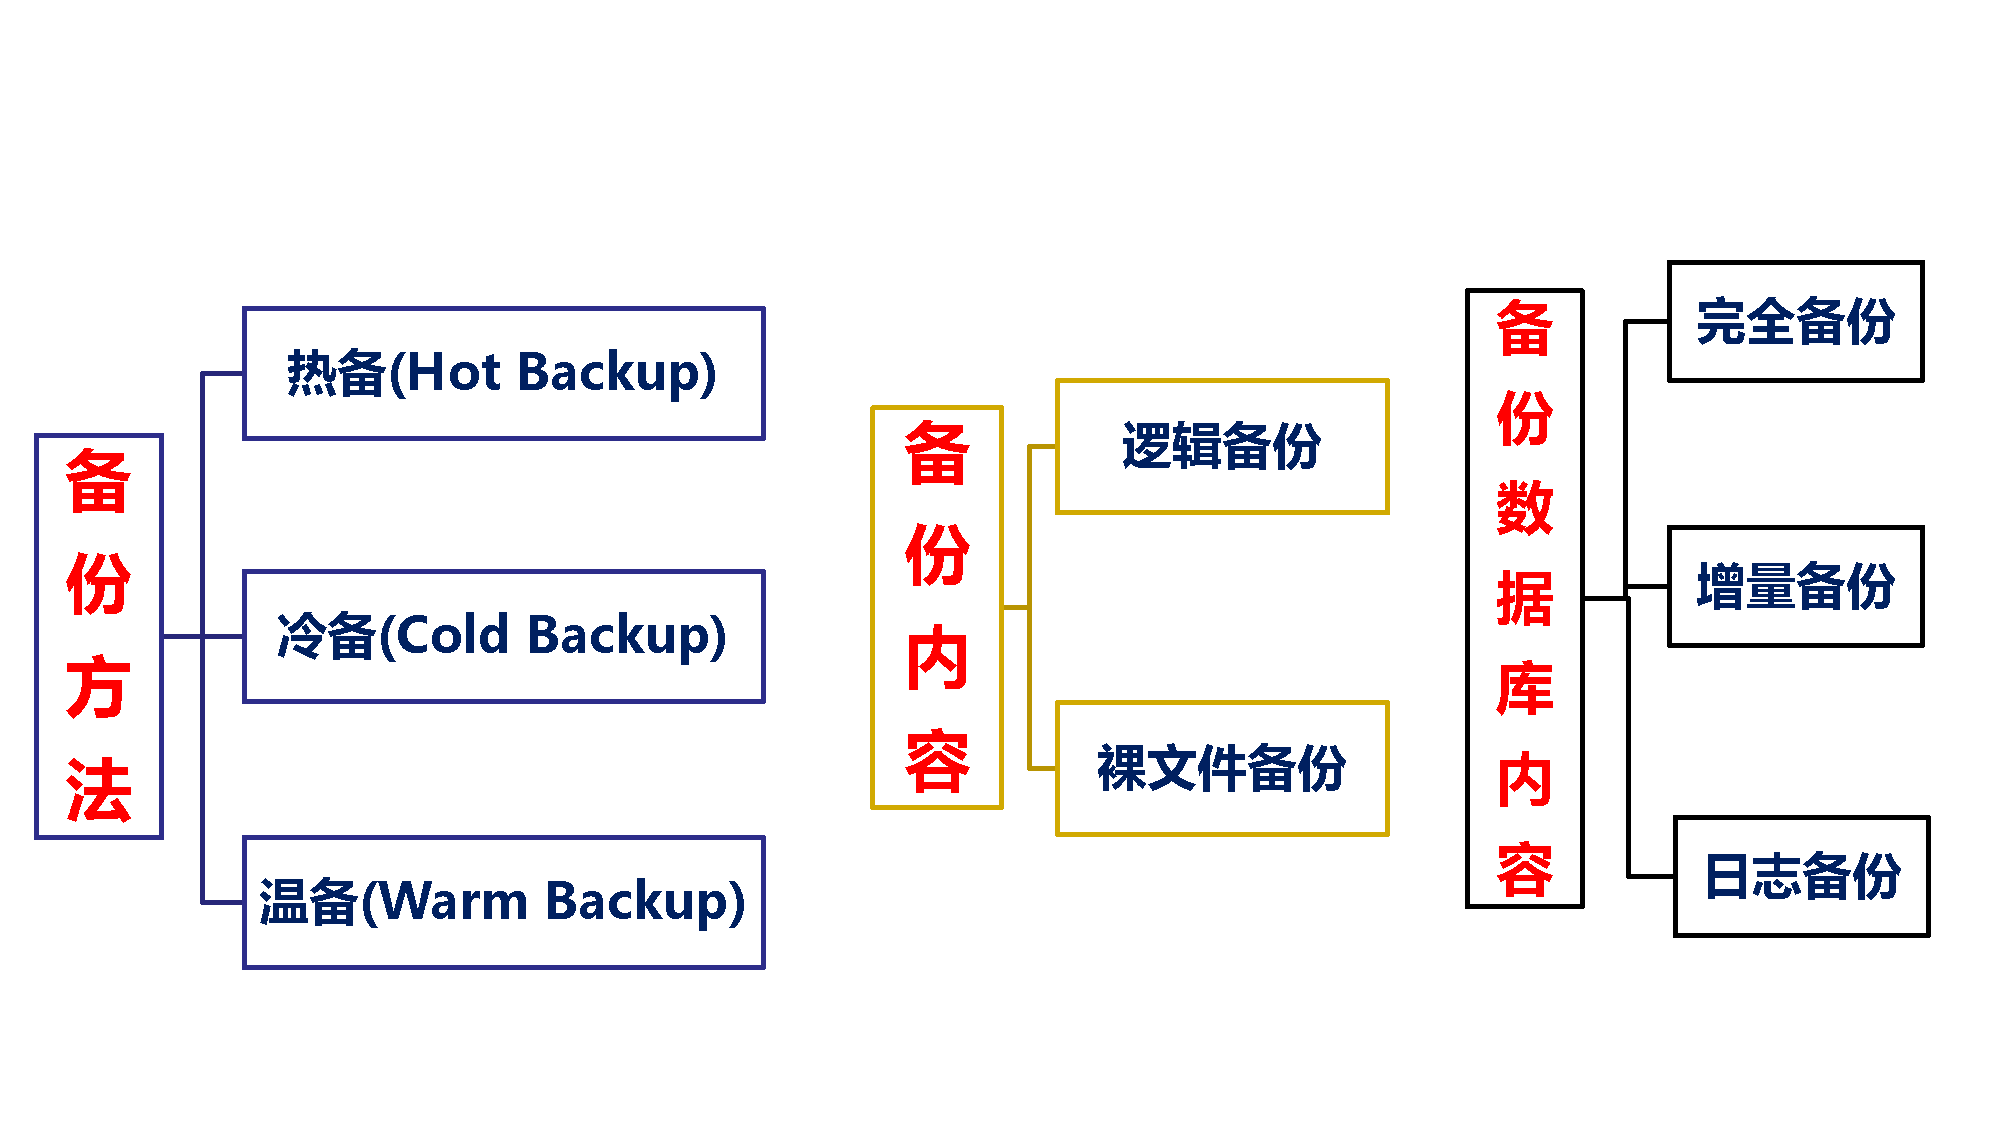
\includegraphics[width=.8\textwidth]{./figure/MySQL备份.pdf}
    \caption{MySQL备份}
\end{figure}

\begin{lstlisting}[language=bash]
# 备份 MySQL 中的所有数据库到一个 SQL 文件中
mysqldump -uroot -p --all-databases > /home/mysql/backups/mysqldump_all_databases.sql

# 备份名为 myDb 的单个数据库
mysqldump -uroot -p myDb > /home/mysql/backups/mysqldump_mydb.sql

# 同时备份两个数据库 myDb1 和 myDb2
mysqldump -uroot -p --databases myDb1 myDb2 > /home/mysql/backups/mysqldump_databases_mydb12.sql

# 备份数据库 myDb 中的单张表 myTb
mysqldump -uroot -p myDb myTb > /home/mysql/backups/mysqldump_myTb.sql

# 备份 myDb 数据库中的 myTb 表,并且只导出 id <= 10 的记录
mysqldump -uroot -p --databases myDb --tables myTb --where="id <= 10" > /home/mysql/backups/mysqldump_myTb10.sql

# 仅备份 db1 和 db2 的数据库结构(不包含数据)
mysqldump --no-data --databases db1 db2 > /home/mysql/backups/structure.sql

# 在 MySQL 客户端中使用 source 恢复全库备份
source /home/mysql/backups/mysqldump_all_databases.sql

# 使用 mysql 命令导入之前备份的 myDb 数据库
mysql -uroot -p myDb < /home/mysql/backups/mysqldump_myDb.sql
\end{lstlisting}

\begin{lstlisting}[language=sql]
-- 把数据库 my_table 中的数据导出到 data.txt 文件中
select * into outfile 'data.txt'
fields terminated by ','
lines terminated by '\r\n'
from my_table;

-- 把 data.txt 文件中的数据导入到 my_table 中
load data infile 'data.txt'
into table my_table
fields terminated by ','
lines terminated by '\r\n';
\end{lstlisting}

下面是用于自动备份多个数据库的 Bash 脚本, 并设置了定时任务(通过 crontab)每天凌晨 3 点执行一次.
\begin{lstlisting}[language=bash]
#!/bin/bash
cd /usr/local/mysql/backup/scripts/
backup_date=`date +%Y%m%d`
filename=/home/db/mysql/backups/databackup_$backup_date.sql
mysql -e "show databases;" -uroot -proot | grep -E "myDb*" | xargs mysqldump -uroot -proot --databases > $filename
echo 'databases backup successfully...'
crontab -e
00 03 * * * /usr/local/mysql/backup/scripts/databases_backup.sh
\end{lstlisting}

\section{日志}

\begin{definition}[日志]
日志文件是以事务为单位用来记录数据库的每一次更新活动的文件, 由系统自动记录.

日志内容包括: 记录名、旧记录值、新记录值、事务标识符、操作标识符等.
\begin{enumerate}
    \item 事务$T_i$开始时, 写入日志: $\langle T_i\ \text{start} \rangle$.
    \item 事务$T_i$执行$\text{write}(X)$之前, 写入日志: $\langle T_i, X, V_1, V_2 \rangle$, 其中$V_1$为更新前的值(前像), $V_2$为更新后的值(后像).
    \item 事务$T_i$提交时, 写入日志: $\langle T_i\ \text{commit} \rangle$.
\end{enumerate}
\end{definition}

根据日志可把事务分为:
\begin{enumerate}
    \item \textcolor{red}{圆满事务}: 日志文件中记录了事务的commit标识.
    \item \textcolor{blue}{夭折事务}: 日志文件中只有start标识, 没有记录事务的commit标识.
\end{enumerate}

基本的恢复操作:
\begin{enumerate}
    \item 对圆满事务的更新日志执行redo操作, 即重新执行该操作, 修改对象被赋予新记录值. 幂等性: $\text{redo}=\text{redo}^2$.
    \item 对夭折事务的更新日志执行undo操作, 即撤销该操作, 修改对象被赋予旧记录值. 幂等性: $\text{undo}=\text{undo}^2$.
\end{enumerate}

其他日志恢复技术: 提交日志(Commit Logging)
\begin{enumerate}
    \item 事务提交之前, 其修改结果不会写入磁盘
    \item 日志中没有提交标记的事务, 其修改结果没有写盘
    \item 恢复时只需重做日志中的提交事务
    \item OceanBase、Hekaton(SQL Server 内存存储引擎)
\end{enumerate}

无日志恢复技术: Shadow Paging.
\begin{enumerate}
    \item 被修改的数据会同时存在两份, 一份是原来的数据, 另一份是修改后的数据(影子, shadow).
    \item 通过两个目录结构分别指向修改前的数据和修改后的数据, 最后Current指针原子切换到新的目录上, 表示事务提交成功.
    \item 当事务提交时, 以一次原子数据写入让整个事务新的修改生效.
\end{enumerate}

\begin{figure}[H]
    \centering
    \begin{minipage}[b]{0.49\linewidth}
    \centering
    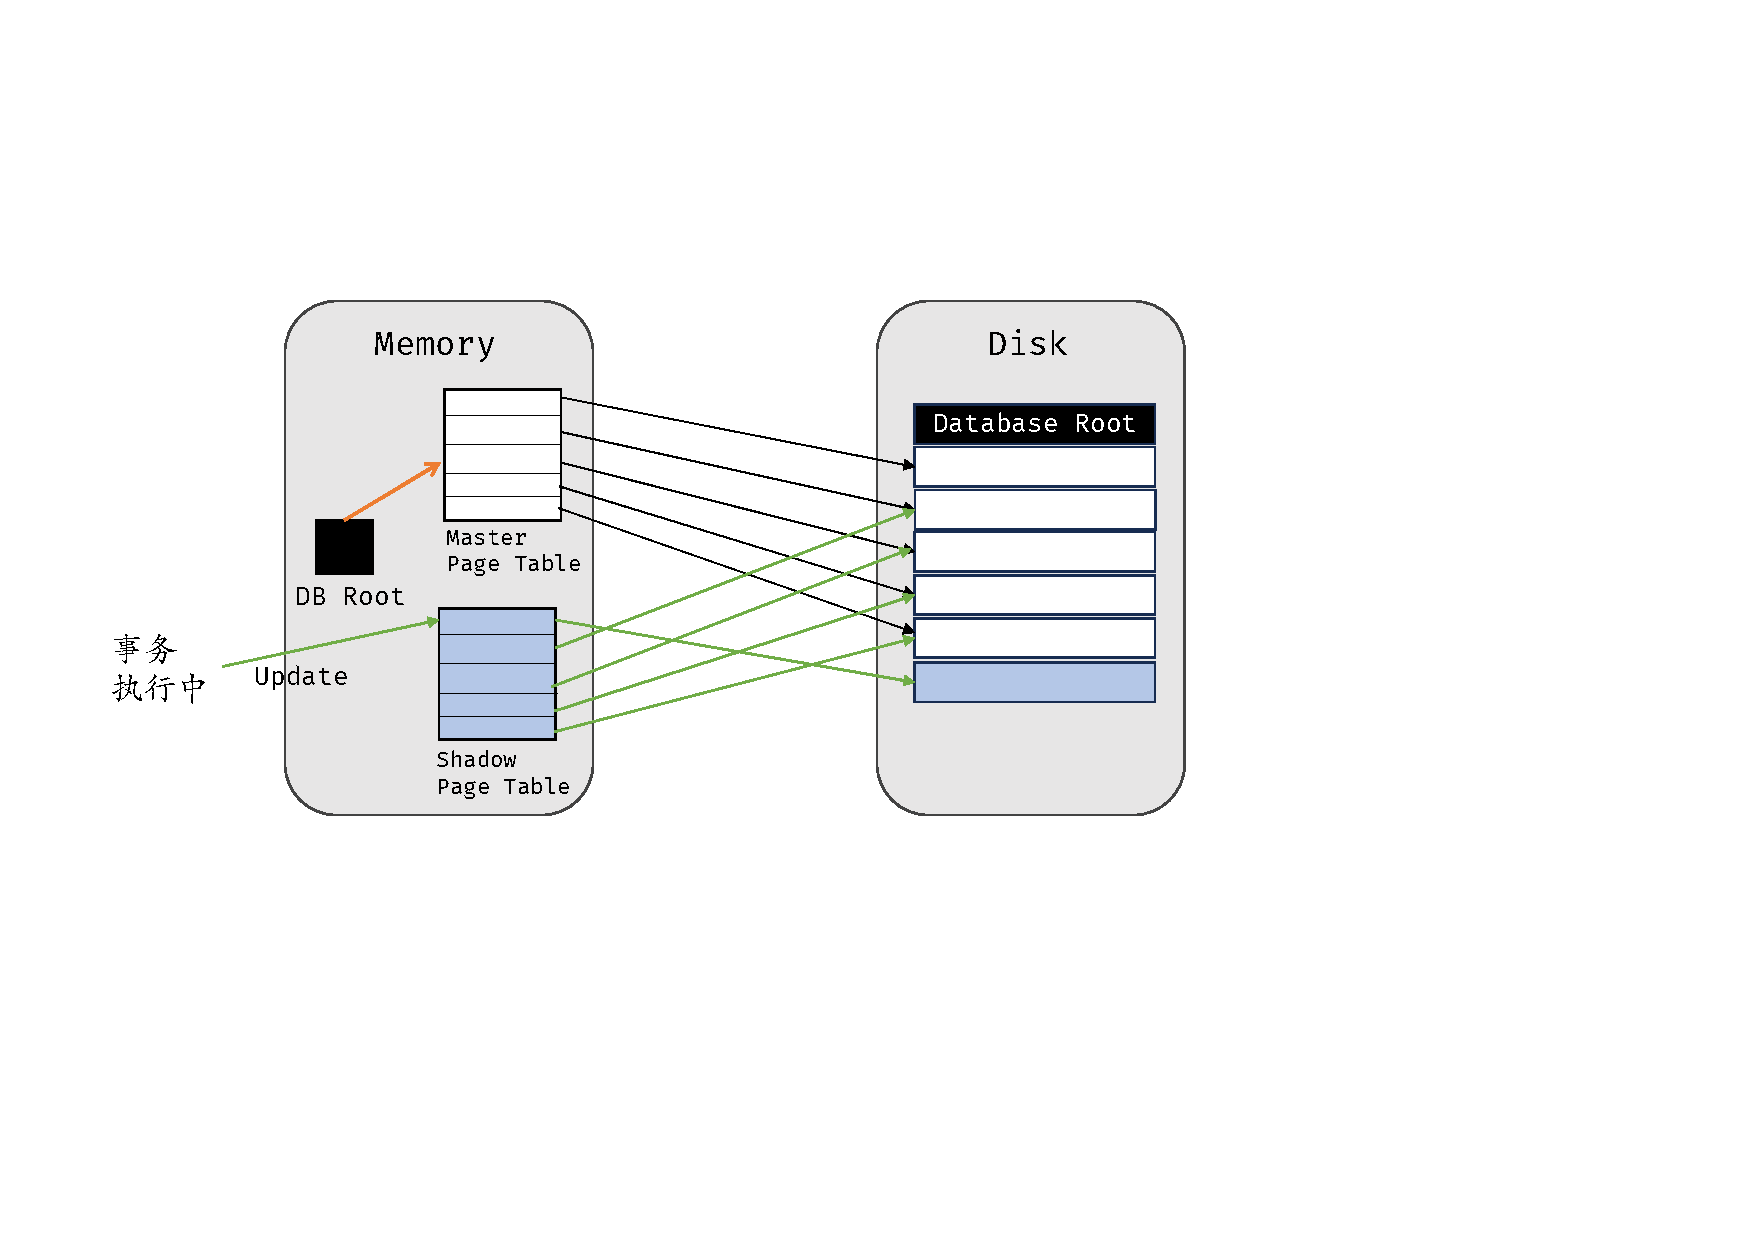
\includegraphics[width=\textwidth]{./figure/shadow-1.pdf}
    \caption{Shadow Paging: 正在修改的事务}
    \end{minipage}
    \hfill
    \begin{minipage}[b]{0.49\linewidth}
    \centering
    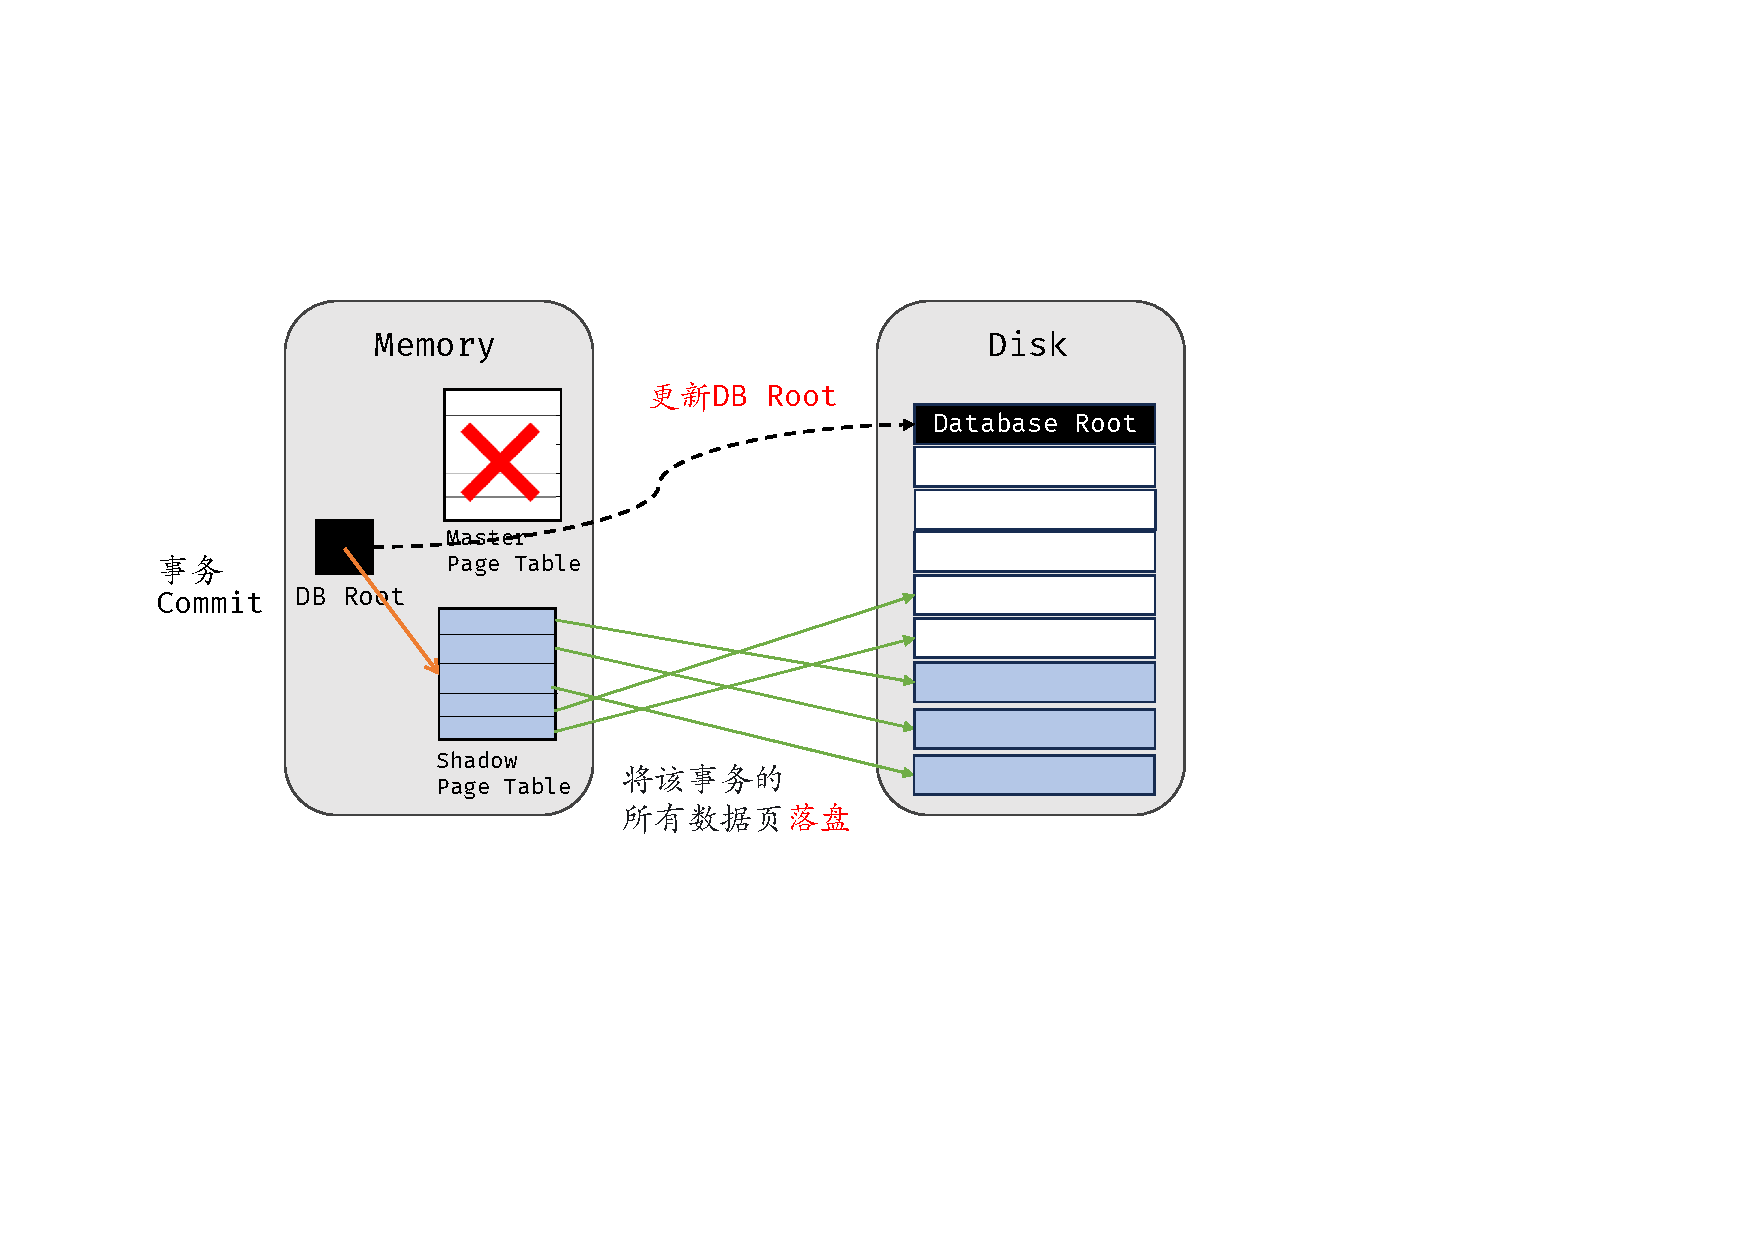
\includegraphics[width=0.95\textwidth]{./figure/shadow-2.pdf}
    \caption{Shadow Paging: 事务Commit}
    \end{minipage}
\end{figure}

Undo/Rollback: 删除 shadow pages (table), 啥都不用做.

Redo: 不需要 redo, 因为每次写事务都会将数据落盘.


MySQL日志文件:
\begin{enumerate}
    \item 重做日志(redo log)
    \item 回滚日志(undo log)
    \item 二进制日志(binary log)
    \item 错误日志(error log)
    \item 慢查询日志(slow query log)
    \item 一般查询日志(general log)
    \item 中继日志(relay log)
\end{enumerate}

慢查询日志的例子:
\begin{lstlisting}[language=sql]
-- 开启慢查询日志功能(1 表示开启)
SET GLOBAL slow_query_log = 1;

-- 设置慢查询日志文件的保存路径(Windows 系统下路径为 C:\slow_statement.log)
-- 注意:MySQL 进程必须对该路径有写入权限
SET GLOBAL slow_query_log_file = 'C:\\slow_statement.log';

-- 设置慢查询时间阈值为 10 秒
-- 所有执行时间超过 10 秒的 SQL 查询会被记录到慢查询日志中
SET GLOBAL long_query_time = 10;

-- 设置慢查询日志输出方式为文件(FILE),也可以设置为 TABLE(表)
SET GLOBAL log_output = 'FILE';

-- 测试语句:执行一个耗时较长的操作,用于触发慢查询日志记录
-- 此处重复执行 MD5('mysql') 函数 99,999,999 次,模拟耗时操作
-- 如果该查询执行时间超过 long_query_time(10秒),则会被记录到慢查询日志中
SELECT BENCHMARK(99999999, MD5('mysql'));
\end{lstlisting}

事务日志是自上次备份事务日志后对数据库执行的所有事务记录, 它可以将数据库恢复到特定时点或恢复到故障点.
\begin{lstlisting}[language=sql]
-- 1. 对数据库 MyDB 执行完整备份,备份到备份设备 MyDB_1
-- 完整备份是所有其他备份(差异、日志)的基础
BACKUP DATABASE MyDB TO MyDB_1;

-- 2. 对数据库 MyDB 执行事务日志备份,备份到备份设备 MyDB_log1
-- 此时会截断日志,并记录从上一次备份以来的所有事务日志
BACKUP LOG MyDB TO MyDB_log1;

-- 3. 再次对数据库 MyDB 执行事务日志备份,备份到备份设备 MyDB_log2
-- 使用 WITH NO_TRUNCATE 表示不截断事务日志,允许后续继续备份
-- 注意:一般只在紧急情况下使用,避免日志文件无限增长
BACKUP LOG MyDB TO MyDB_log2 WITH NO_TRUNCATE;

-- 4. 恢复完整备份,从备份设备 MyDB_1 还原数据库 MyDB
-- 使用 WITH NORECOVERY 表示数据库仍处于还原状态,等待后续日志应用
RESTORE DATABASE MyDB FROM MyDB_1 WITH NORECOVERY;

-- 5. 应用第一个事务日志备份 MyDB_log1
-- 仍然使用 WITH NORECOVERY,表示还有更多日志需要恢复
RESTORE LOG MyDB FROM MyDB_log1 WITH NORECOVERY;

-- 6. 应用第二个事务日志备份 MyDB_log2
-- 使用 WITH RECOVERY 表示这是最后一次恢复操作,数据库将变为可用状态
RESTORE LOG MyDB FROM MyDB_log2 WITH RECOVERY;
\end{lstlisting}

with norecovery: 重做所有日志记录.

with recovery: 回滚失败事务日志记录

\begin{example}
事务$T$从A账户过户¥50到B账户:
\begin{align*}
    &\text{read}(A); A :=  A - 50; \text{write}(A) \\
    &\text{read}(B); B :=  B + 50; \text{write}(B) \\
    &\text{commit}(T)
\end{align*}

MyDB\_log1: $\langle T, A, 100, 50 \rangle$.

MyDB\_log2: $\langle T, B, 100, 150 \rangle, \langle T, \text{commit} \rangle$.

下面各自恢复结果是什么:
\begin{lstlisting}[language=SQL]
restore log MyDB from MyDB_log1 with norecovery
restore log MyDB from MyDB_log2 with recovery
\end{lstlisting}

\begin{lstlisting}[language=SQL]
restore log MyDB from MyDB_log1 with recovery
restore log MyDB from MyDB_log2 with recovery
\end{lstlisting}
\end{example}

第一种情况: 应用日志MyDB\_log1, 只执行了对A账户的更新操作, B账户没有更新, 事务未提交, 所以B账户的余额仍然是100. 数据库仍处于RESTORING 状态. 接着应用日志MyDB\_log2, 执行了对B账户的更新操作, 由于事务已经提交, 所以B账户的余额被更新为150.

第二种情况: 应用日志MyDB\_log1, 只执行了对A账户的更新操作, B账户没有更新, 事务未提交, 所以B账户的余额仍然是100. 现在完成恢复过程并且发布数据库了. 但是是不完整的log, 需要回滚. 同时已经恢复了, 无法再restore了. 最后A和B都没有改变.

恢复模型: SQL Server
\begin{enumerate}
    \item 简单恢复模型: 允许将数据库恢复到最新的备份. 数据库备份 + 差异备份(可选)
    \item 完全恢复: 允许将数据库恢复到故障点状态. 数据库备份 + 差异备份(可选) + 事务日志备份.
    \item 大容量日志记录恢复: 允许大容量日志记录操作(bulk insert...). 数据库备份 + 差异备份(可选) + 事务日志备份.
\end{enumerate}

\section{WAL, Write Ahead Log}

WAL 的中文名是预写日志系统, 其核心思想是把用户所有的修改操作(插入、删除)先写入日志中, 
然后再应用到系统状态里. 
一旦成功写完日志, 即可通知用户操作成功. 
由于日志是以尾部追加方式写入, 耗时较短, 所以不会长时间阻塞用户线程.
此外为防止意外退出导致数据丢失, 系统重启时还会根据日志重做用户操作, 以保证数据可靠性.

\textbf{为什么不能先写数据库?}

如果先写DB, 则可能在写的中途发生系统崩溃, 导致内存缓冲区内容丢失,
而外存DB处于不一致状态, 由于日志缓冲区内容已破坏, 导致无法对DB恢复.

\textbf{WAL总可以保证恢复的一致性!!!}

\textcolor{red}{日志缓冲区和数据库缓冲区的写时机不同:}
\begin{enumerate}
    \item 同步(synchronous)写日志: 只有事务的相关日志已经完全在磁盘上了, 才会向进程发送该事务已提交的确认消息.
    \item 异步(asynchronous)写缓冲区: 只需要将数据页的写入操作投递给操作系统即可, 不需要等待其完成.
\end{enumerate}

\begin{figure}[H]
    \centering
    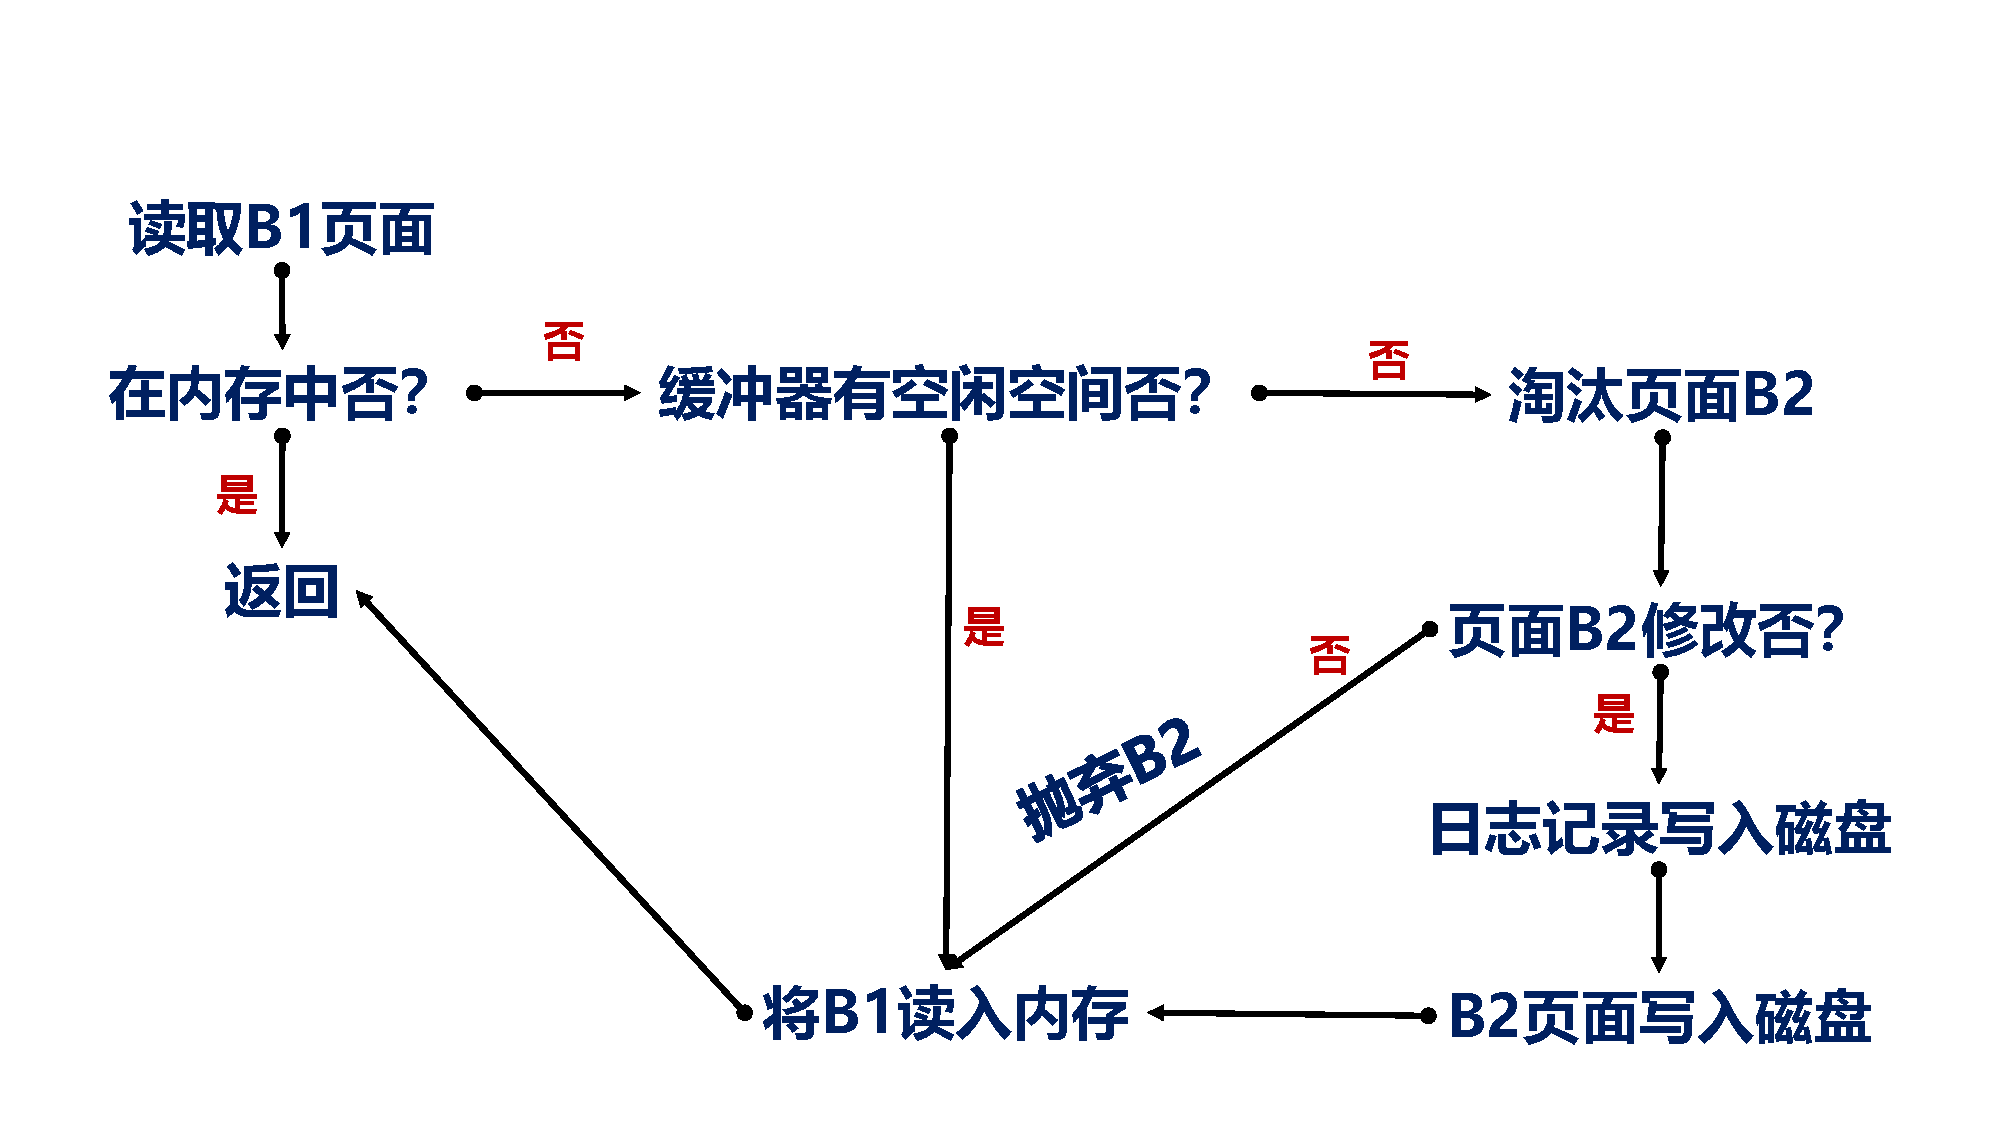
\includegraphics[width=.6\textwidth]{figure/读写页面.pdf}
    \caption{读取一个页面的过程 (actually from 操作系统)}
\end{figure}

在主线程每秒一次的循环中, 将undo log缓冲器的内容刷新到重做日志文件中, 即便某个事务尚未提交.
由参数\textcolor{red}{innodb\_flush\_log\_at\_trx\_commit}控制.
\begin{itemize}
    \item 0 代表提交事务时, 并不立即刷出日志, 而是等待主线程每秒的刷新;
    \item 1 代表提交事务时, 将undo log同步写磁盘, 也即伴有fsync()的调用;
    \item 2 代表提交事务时, 将undo log异步写磁盘, 也即写入文件系统缓存中.
\end{itemize}

fsync是昂贵操作, MySQL一次事务提交最多会导致3次fsync.

将多个并发提交的事务共享一次fsync操作:
\begin{itemize}
    \item binlog\_group\_commit\_sync\_delay = N: 在等待N微秒后, 进行binlog刷盘操作
    \item binlog\_group\_commit\_sync\_no\_delay\_count = N: 达到最大事务等待数量, 开始binlog刷盘
\end{itemize}

\section{故障恢复}

\subsection{事务故障恢复}

\textcolor{red}{事务故障恢复过程: 撤消事务已对数据库所做的修改}
\begin{itemize}
    \item 反向扫描日志文件, 查找该事务的更新操作
    \item 对事务更新操作执行undo操作, 即将事务更新前的旧值写入数据库
    \item 继续反向扫描日志文件, 查找该事务的其他更新操作, 并做同样处理
    \item 直至读到事务的开始标识, 结束事务故障恢复过程
\end{itemize}
为什么同一事务的日志记录需要反向链接在一起? 加快撤销速度.

反向undo: 保持一致性.

\subsection{系统故障恢复}

\textcolor{red}{系统故障造成不一致状态的原因}
\begin{itemize}
    \item 未完成事务对数据库的更新已写入数据库
    \item 已提交事务对数据库的更新未写入数据库
\end{itemize}

\textcolor{red}{系统故障恢复过程}:
\begin{itemize}
    \item 正向扫描日志文件, 将圆满事务记入重做队列, 将夭折事务记入撤消队列;
    \item 反向扫描日志, 对撤消队列中事务$T_i$的每条日志记录执行undo操作;
    \item 正向扫描日志文件, 对重做队列中事务$T_i$的每条日志记录执行redo操作.
\end{itemize}

\subsection{介质故障恢复}

\textcolor{red}{介质故障恢复过程}:
\begin{itemize}
    \item 装入最新的数据库后备副本, 使数据库恢复到最近一次转储时的一致性状态;
    \item 装入相应的日志文件副本, 重做已完成的事务.
\end{itemize}

\begin{figure}[H]
    \centering
    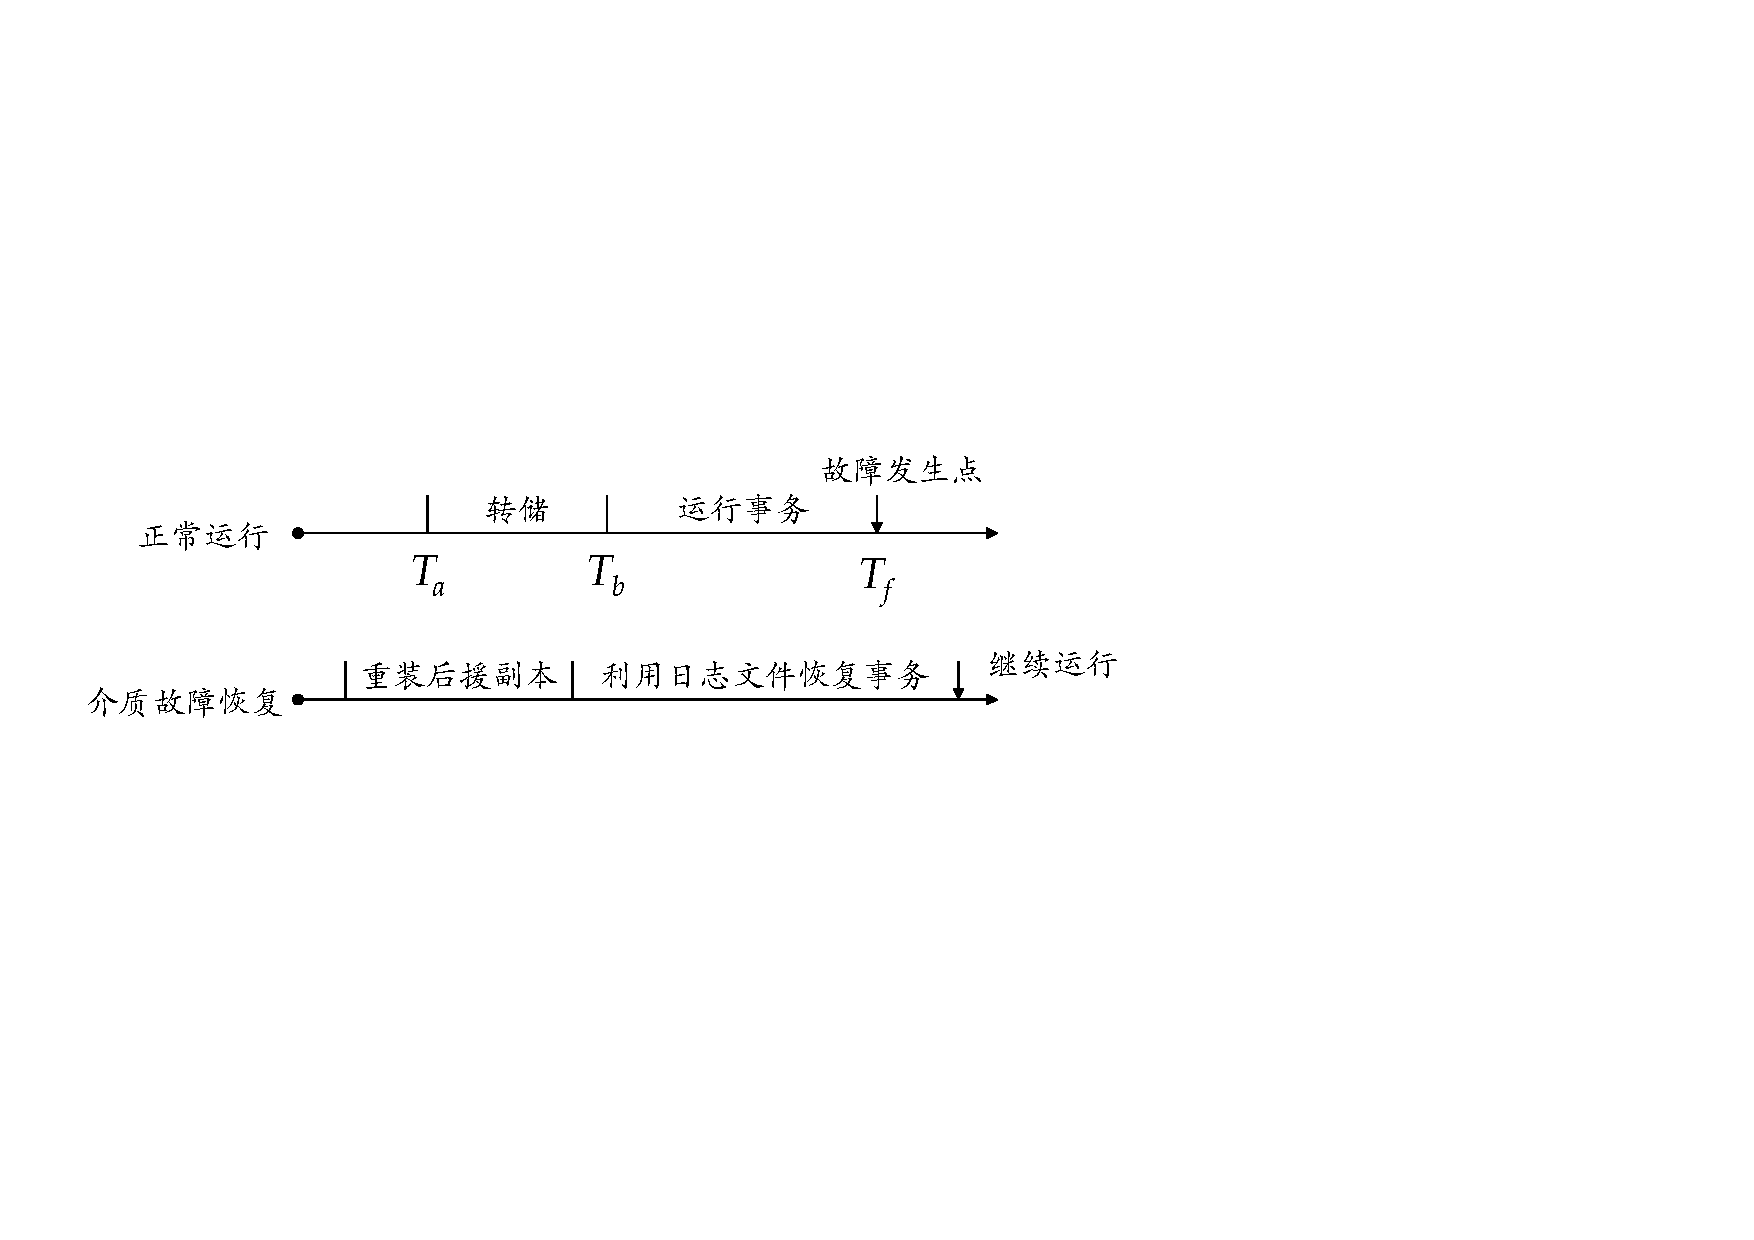
\includegraphics[width=.6\textwidth]{figure/介质故障.pdf}
    \caption{介质故障恢复过程}
\end{figure}

\section{检查点(Checkpoint)}

如何减少\textbf{系统故障恢复}过程中必须重做的事务数量?
\begin{itemize}
    \item 当发生系统故障时, 我们必须搜索整个日志, 以决定哪些事务需要redo, 哪些需要undo
    \item 大多数需要被重做的事务其更新已经写入了数据库中($\text{redo}^2$)
    \item 尽管对它们重做不会造成不良后果, 但会使恢复过程变得更长
\end{itemize}

如何确保已提交事务的结果已经写入数据库了?
\begin{itemize}
    \item 保证在检查点时刻磁盘上日志文件与数据库的内容是一致的(就像Ctrl+S一样)
\end{itemize}

\begin{figure}[H]
    \centering
    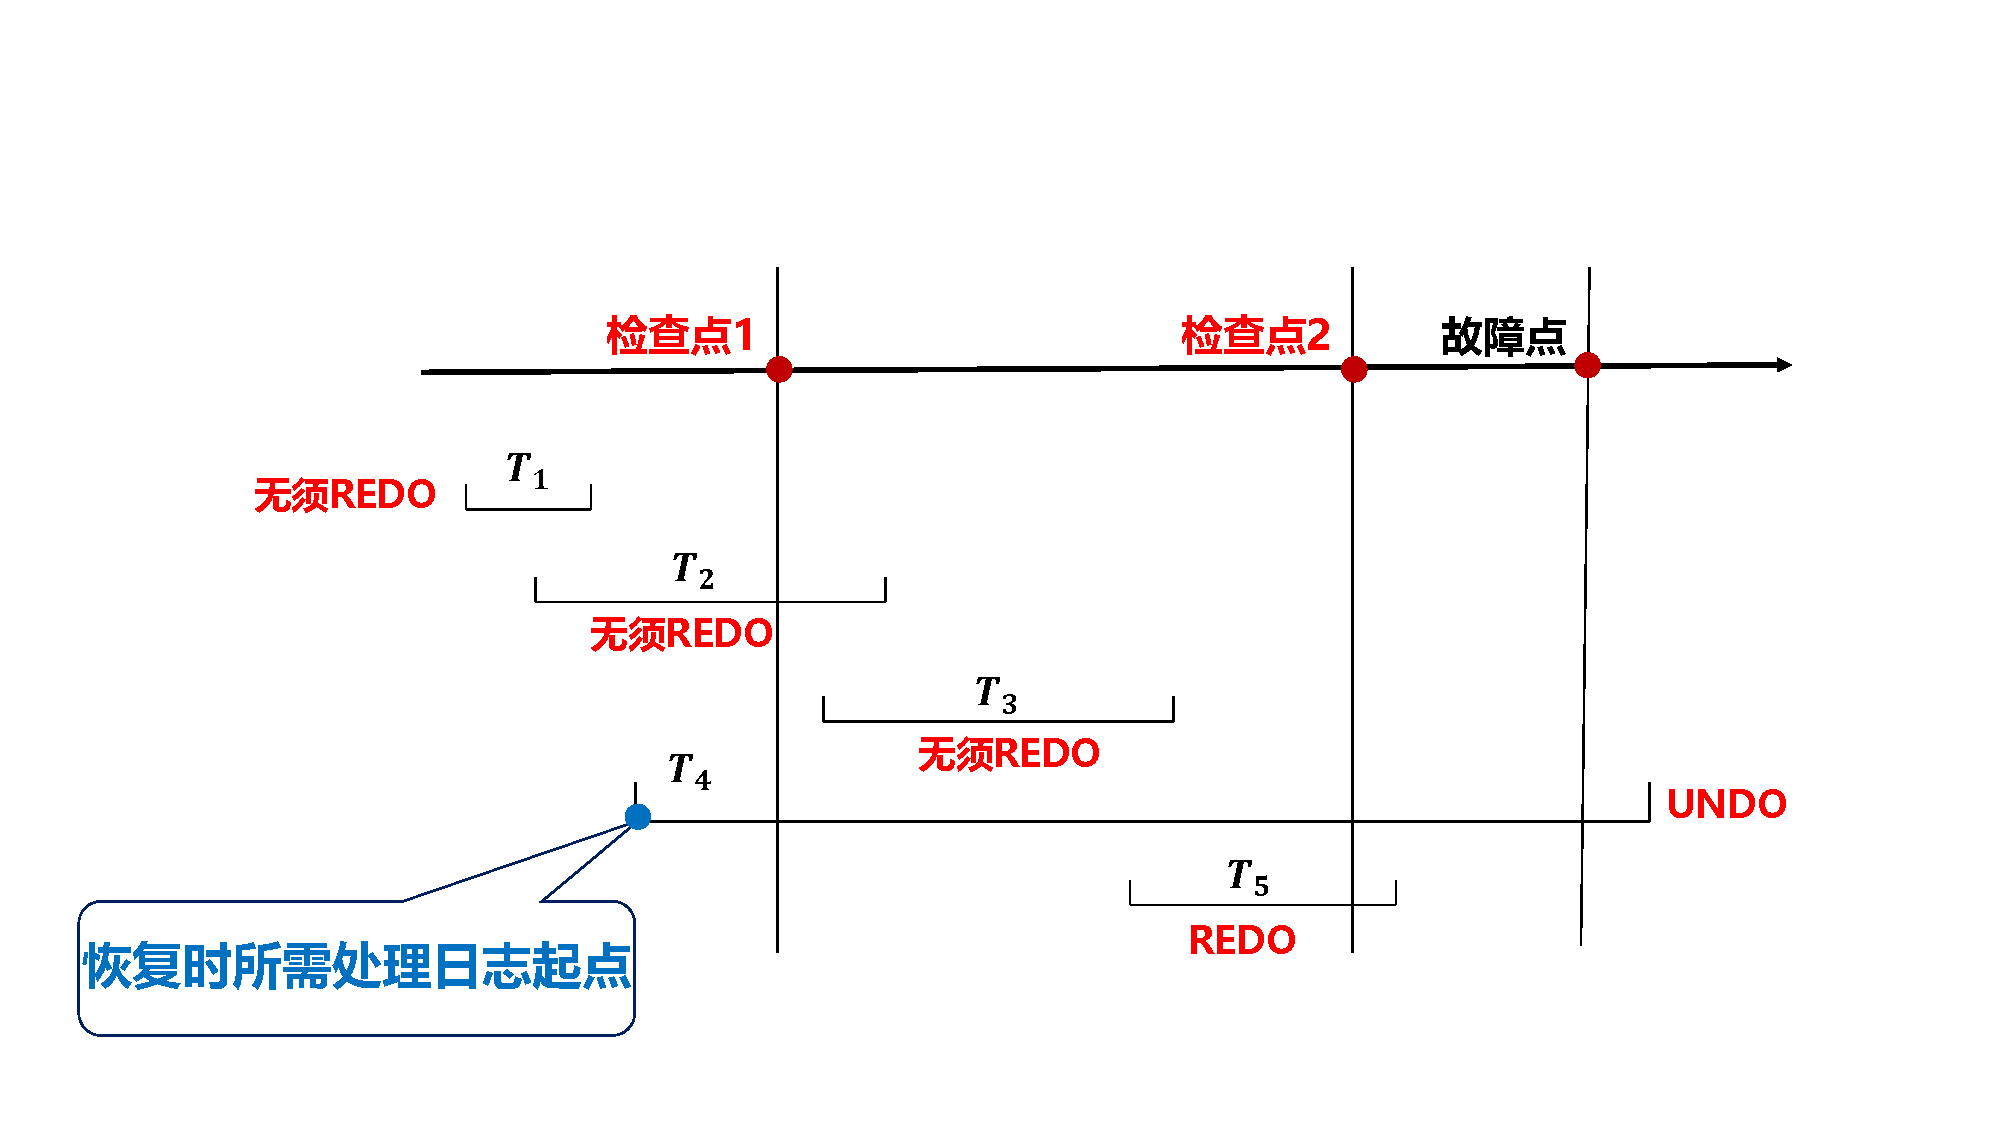
\includegraphics[width=.7\textwidth]{figure/检查点.pdf}
    \caption{检查点在系统故障恢复中的作用}
\end{figure}

一致性检查点: Consistent Checkpoint

模糊检查点: Fuzzy Checkpoint

"Unimport. There's a million things I haven't done."


\section{ARIES恢复算法}

下面介绍ARIES恢复算法\cite{10.1145/128765.128770}.

\begin{figure}[H]
    \centering
    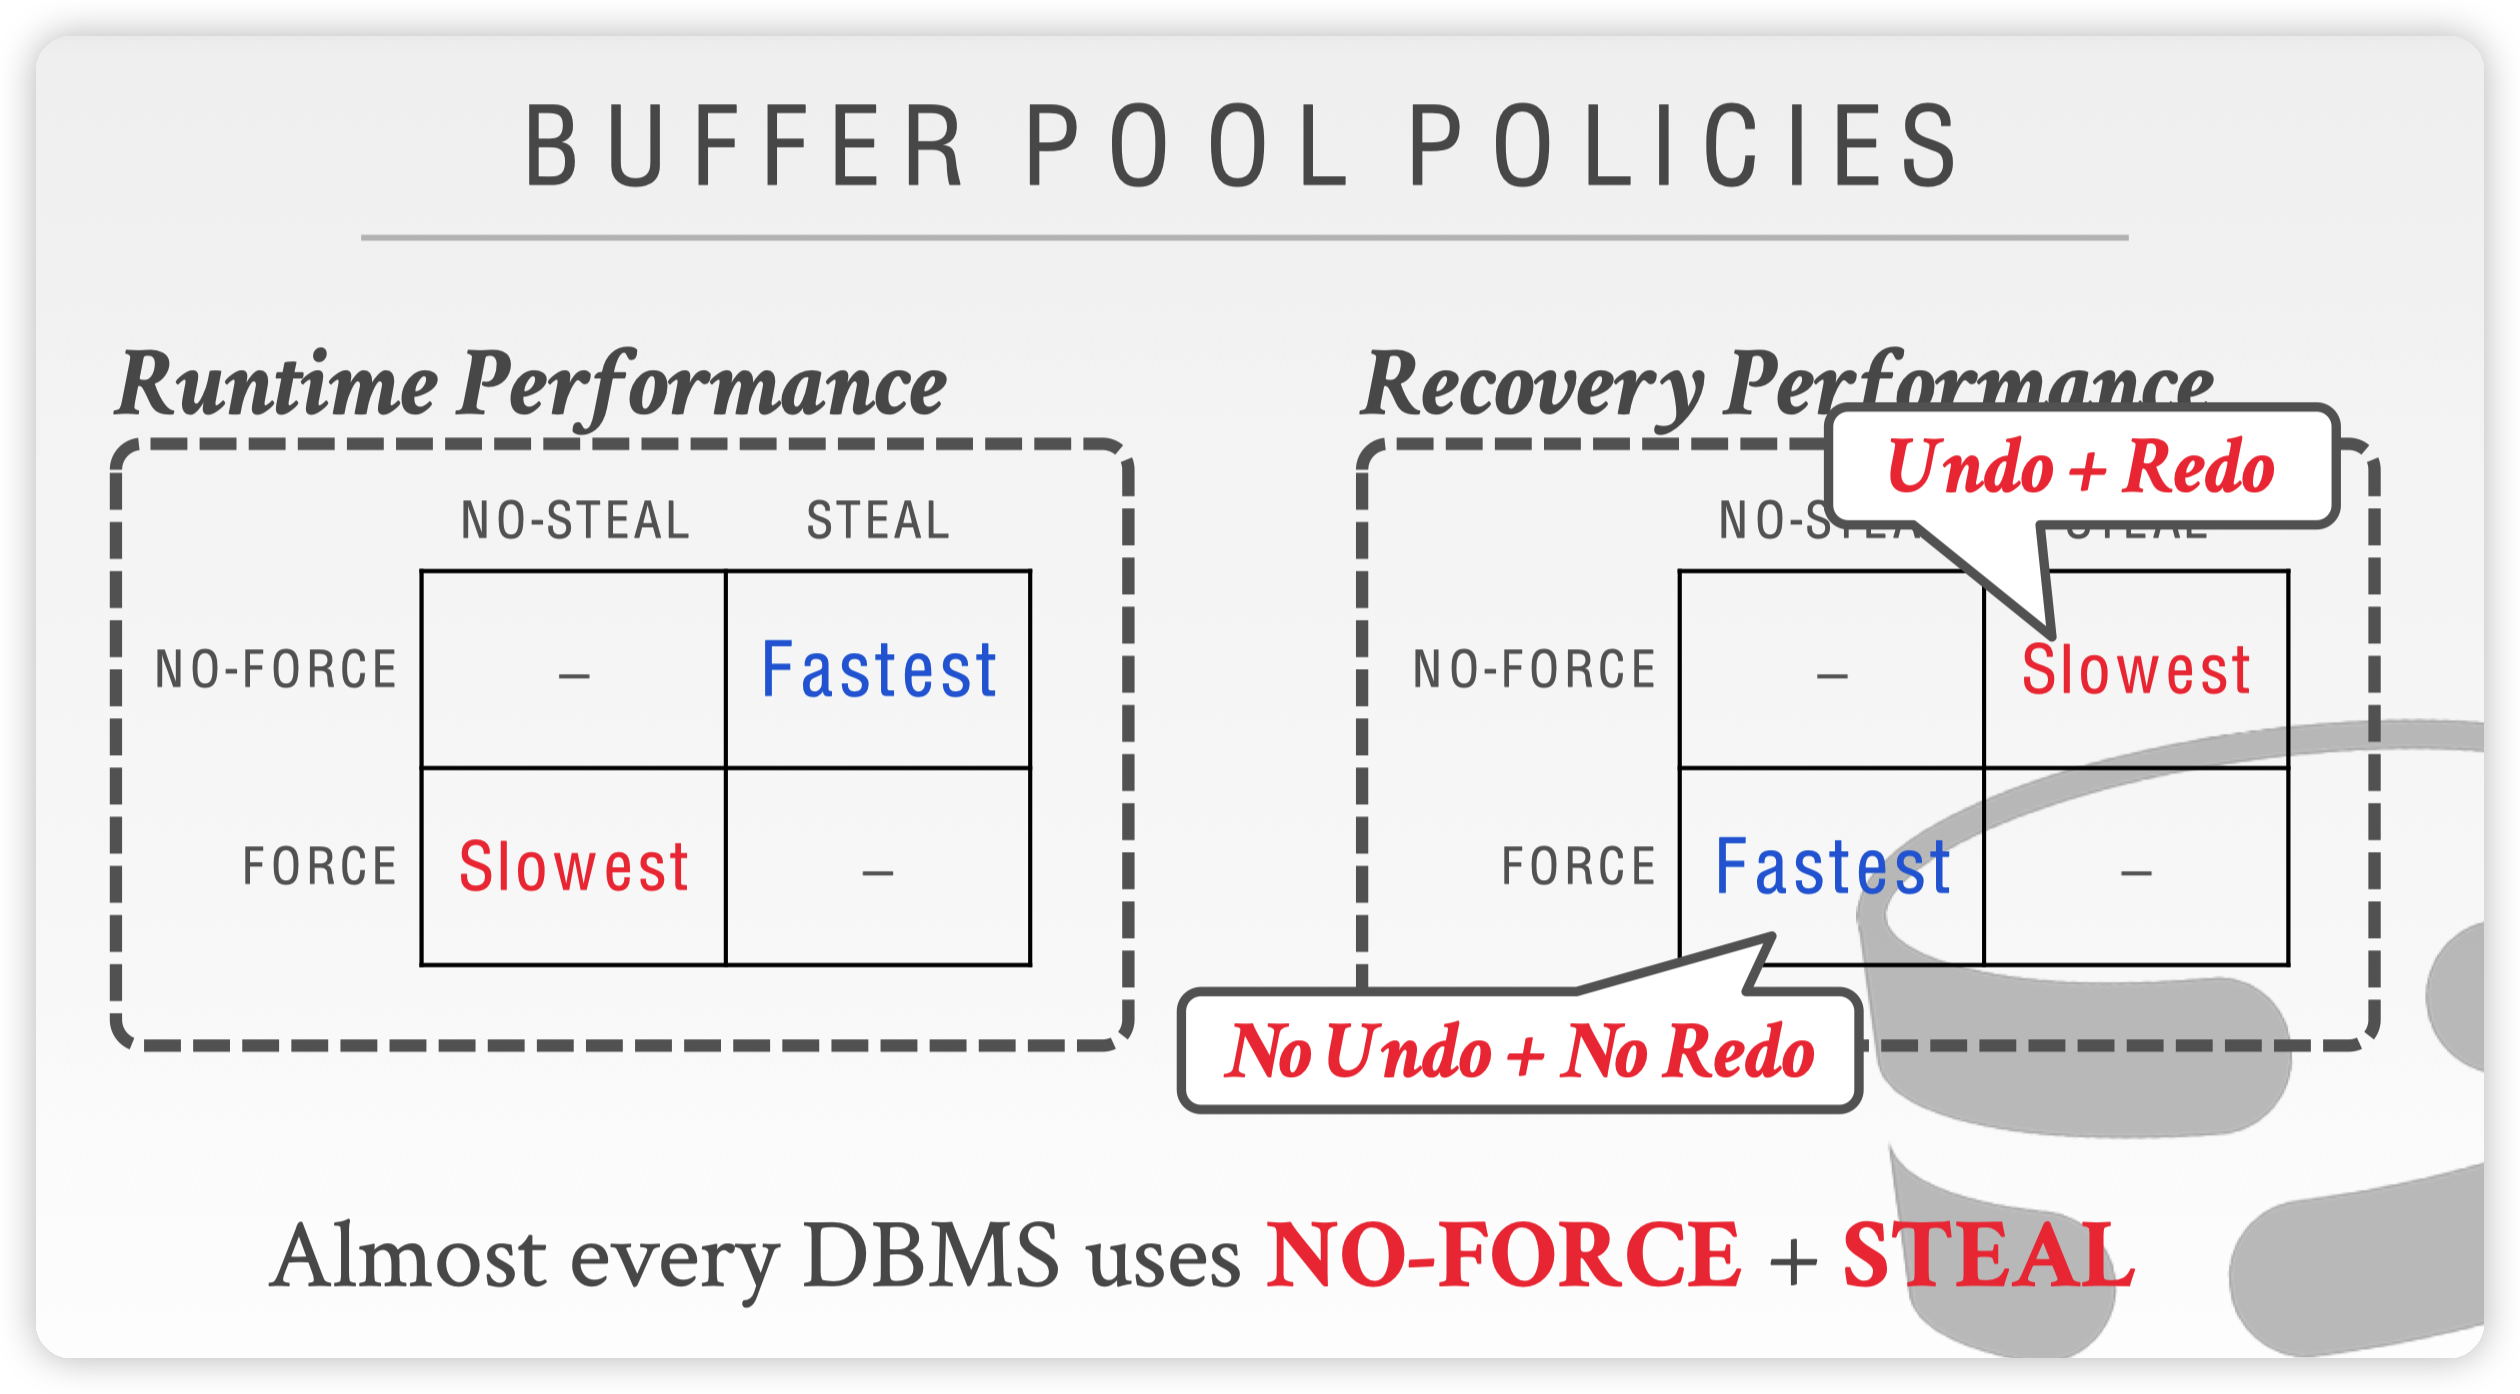
\includegraphics[width=.7\textwidth]{figure/policies.png}
    \caption{Buffer Pool Policies}
\end{figure}


\begin{definition}[Steal Policy]
是否允许未提交事务的修改在持久化存储上生效(Whether the DBMS allows an uncommitted txn to overwrite the most recent committed value of an object in non-volatile storage), 被称为Steal policy.
\begin{itemize}
    \item 允许未提交事务的修改持久化存储上生效 $\to$ Steal policy.
    \item 不允许 $\to$ No Steal Policy.
\end{itemize}
\end{definition}

\begin{definition}[Force Policy]
一个事务在提交之前是否需要将所有修改同步到持久化存储上(Whether the DBMS requires that all updates made by a txn are reflected on non-volatile storage before the txn is allowed to commit.)
\begin{itemize}
    \item 必须将事务的所有修改都同步到持久化存储上, 事务才被允许提交 $\to$ Force policy.
    \item 不必 $\to$ No force policy.
\end{itemize}
\end{definition}

ARIES算法也是no force + steal.


